% Please make sure you insert your
% data according to the instructions in PoSauthmanual.pdf
\documentclass[a4paper,11pt]{article}
\usepackage{pos}
\usepackage{sidecap}    
\sidecaptionvpos{figure}{m}    
\sidecaptionvpos{table}{m}    
\usepackage{cleveref}    
\usepackage{enumitem}
\setitemize{itemsep=0pt,parsep=1pt,topsep=1pt,itemindent=0pt,leftmargin=9pt}    
\setenumerate{itemsep=0pt,parsep=1pt,topsep=1pt,itemindent=10pt,leftmargin=9pt}    
\usepackage{natbib}    
\setlength{\bibsep}{2pt}    
\setlength{\parindent}{0pt}    

\usepackage{listings}

\definecolor{codegreen}{rgb}{0,0.6,0}
\definecolor{codegray}{rgb}{0.5,0.5,0.5}
\definecolor{codepurple}{rgb}{0.58,0,0.82}
\definecolor{backcolour}{rgb}{0.95,0.95,0.92}

\lstdefinestyle{mystyle}{
    backgroundcolor=\color{backcolour},   
    commentstyle=\color{codegreen},
    keywordstyle=\color{magenta},
    numberstyle=\tiny\color{codegray},
    stringstyle=\color{codepurple},
    basicstyle=\ttfamily\tiny,
    breakatwhitespace=false,
    breaklines=true, 
    captionpos=b,
    keepspaces=true,
    numbers=left,
    numbersep=5pt,
    showspaces=false,
    showstringspaces=false,
    showtabs=false,
    tabsize=2
}

\lstset{style=mystyle}

\usepackage{algorithm}
\usepackage{algorithmicx}
\usepackage{algpseudocode}

\usepackage[font={small,it},labelfont=bf,tableposition=top]{caption}

\newcommand{\tr}{\operatorname{Tr}}
\newcommand{\re}{\operatorname{Re}}
\newcommand{\im}{\operatorname{Im}}
\newcommand{\C}{\mathbb{C}}
\newcommand{\R}{\mathbb{R}}
\newcommand{\ID}{\mathbb{I}}
\newcommand{\rf}{\mathcal{R}_5^{\mathbf{sp}}}
\newcommand{\hQpm}{\hat Q^{\pm}}
\newcommand{\hWpm}{\hat W^{\pm}}
\newcommand{\hQp}{\hat Q^{+}}
\newcommand{\hQm}{\hat Q^{-}}
\newcommand{\hWp}{\hat W^{+}}
\newcommand{\hWm}{\hat W^{-}}
\newcommand{\Wpm}{W^{\pm}}
\newcommand{\Qpm}{Q^{\pm}}
\newcommand{\Qp}{Q^{+}}
\newcommand{\Qm}{Q^{-}}
\newcommand{\Wp}{W^{+}}
\newcommand{\Wm}{W^{-}}
\newcommand{\Qnd}{Q_{\textrm{ND}}}
\newcommand{\Tee}{T_{ee}}
\newcommand{\Too}{T_{oo}}
\newcommand{\Moe}{M_{oe}}
\newcommand{\Moo}{M_{oo}}
\newcommand{\Meo}{M_{eo}}
\newcommand{\Mee}{M_{ee}}
\newcommand{\order}{\mathcal{O}}

\newcommand{\Sg}{S_\mathrm{G}}
\newcommand{\Sdeg}{S_\mathrm{deg}}
\newcommand{\Smusig}{S_{\mu_\sigma}}
\newcommand{\Sdel}{S_\delta}
\newcommand{\mudel}{\mu_\delta}
\newcommand{\musig}{\mu_\sigma}
\newcommand{\mutilsig}{\tilde{\mu}_\sigma}
\newcommand{\mutildel}{\tilde{\mu}_\delta}
\newcommand{\mul}{\mu_\ell}
\newcommand{\D}{\mathcal{D}}
\newcommand{\dtau}{\delta\tau}

\newcommand{\csw}{c_\mathrm{sw}}
\newcommand{\mpcac}{m_\mathrm{PCAC}}
\newcommand{\Ntraj}{N_\mathrm{traj}}
\newcommand{\Nmeas}{N_\mathrm{meas}}
\newcommand{\Nconf}{N_\mathrm{conf}}
\newcommand{\Mpi}{M_{\pi^\pm}}
\newcommand{\Mphyspi}{M_{\pi^\pm}^\mathrm{phys}}
\newcommand{\Fpi}{f_{\pi^\pm}}
\newcommand{\Mpin}{M_{\pi^0}}
\newcommand{\Mpinc}{M_{\pi^{(0,c)}}}
\newcommand{\ld}{\mathrm{(LD)}}
\newcommand{\cd}{\mathrm{(CD)}}

\newcommand{\fnabla}{\nabla^\mathrm{f}}
\newcommand{\bnabla}{\nabla^\mathrm{b}}

\newcommand{\mps}{M_\mathrm{P}}
\newcommand{\ps}{\mathrm{P}}
\newcommand{\mpi}{M_\pi}
\newcommand{\mphyspi}{M_{\pi}^\mathrm{phys}}
\newcommand{\fps}{f_\mathrm{P}}
\newcommand{\fpi}{f_\pi}
\newcommand{\mcrit}{m_\mathrm{crit}}
\newcommand{\mw}{m_\mathrm{W}}
\newcommand{\kc}{\kappa_c}
\newcommand{\mn}{M_\mathrm{N}}
\newcommand{\dof}{\mathrm{dof}}

\newcommand{\lmin}{\lambda_\mathrm{min}}
\newcommand{\lmax}{\lambda_\mathrm{max}}
\newcommand{\qcdlambda}{\Lambda_\mathrm{QCD}}

\newcommand{\chipt}{$\chi$PT}
\newcommand{\wchipt}{W$\chi$PT}
\newcommand{\wtmchipt}{Wtm$\chi$PT}

\newcommand{\dingcircle}{\ding{108}}
\newcommand{\dingsquare}{\ding{110}}
\newcommand{\dingrhombus}{\ding{117}}
\newcommand{\dingtriangle}{\ding{115}}

\newcommand{\mev}{~\mathrm{MeV}}
\newcommand{\gev}{~\mathrm{GeV}}
\newcommand{\fm}{~\mathrm{fm}}

\newcommand{\nmev}{\mathrm{MeV}}
\newcommand{\ngev}{\mathrm{GeV}}
\newcommand{\nfm}{\mathrm{fm}}

\newcommand{\Fav}{\|F\|_\mathrm{av}^2}
\newcommand{\Fmax}{\|F\|_\mathrm{max}^2}
\newcommand{\Fsq}{\|F\|^2}
\newcommand{\mutil}{\tilde{\mu}}
\newcommand{\rhotil}{\tilde{\rho}}
\newcommand{\ctil}{\tilde{c}_\mathrm{sw}}

\newcommand{\talkcite}[1]{{\footnotesize \textcolor{blue}{[#1]}}}

\newcommand{\backupbegin}{
   \newcounter{finalframe}
   \setcounter{finalframe}{\value{framenumber}}
}
\newcommand{\backupend}{
   \setcounter{framenumber}{\value{finalframe}}
}

% full page width float
%   \checkoddpage
%   \edef\side{\ifoddpage l\else r\fi}%
%   \makebox[\textwidth][\side]{%
%   \begin{minipage}{1.35\linewidth}
%   \end{minipage}
%   }%

% margin figure
% \marginpar{
%   \centering
%   \includegraphics[width=\linewidth]{}
%   \captionof{figure}[]{}
%   \label{}
% }

% \newtcolorbox{hpcablock}[2][]{%
%   left=3pt,
%   right=3pt,
%   top=3pt,
%   bottom=3pt,
%   colback=bg,
%   colframe=structure!100,
%   fonttitle=\sffamily,
%   coltitle=structure!100,
%   colbacktitle=structure!10,
%   enhanced,
%   attach boxed title to top,
%   title=#2,
%   #1}

% \newtcolorbox{hpcaexampleblock}[2][]{%
%   left=3pt,
%   right=3pt,
%   top=3pt,
%   bottom=3pt,
%   colback=bg,
%   colframe=example text.fg!100,
%   fonttitle=\sffamily,
%   coltitle=example text.fg!100,
%   colbacktitle=example text.fg!10,
%   enhanced,
%   attach boxed title to top left,
%   title=#2,
%   #1}

% \newtcolorbox{hpcaalertblock}[2][]{%
%   left=3pt,
%   right=3pt,
%   top=3pt,
%   bottom=3pt,
%   colback=bg,
%   colframe=alert!100,
%   fonttitle=\sffamily,
%   coltitle=alert!100,
%   colbacktitle=alert!10,
%   enhanced,
%   attach boxed title to top left,
%   title=#2,
%   #1}


\title{Status of the ETMC ensemble generation effort}
%% \ShortTitle{Short Title for header}

\author[a,b]{C.~Alexandrou}
\author[b]{S.~Bacchio}
\author[c]{J.~Finkenrath}
\author[d]{R.~Frezzotti}
\author*[e]{M.~Garofalo}
\author*[e]{B.~Kostrzewa}
\author[b]{G.~Koutsou}
\author[f]{S.~Romiti}
\author[e]{A.~Sen}
\author[e]{C.~Urbach}
\author[f]{U.~Wenger}

\affiliation[a]{Department of Physics, University of Cyprus, 20536 Nicosia, Cyprus}
\affiliation[b]{Computation-based Science and Technology Research Center, The Cyprus Institute, 2121 Nicosia, Cyprus}
\affiliation[c]{Theoretical Physics Department, CERN 1211 Geneva 23, Switzerland}
\affiliation[d]{Dipartimento di Fisica and INFN, Universit{\`a} di Roma ``Tor Vergata'', I-00133}
\affiliation[e]{Helmholtz-Institut für Strahlen und Kernphysik (Theory), Rheinische Friedrich-Wilhelms-Universität Bonn, Nussallee 14-16, 53115 Bonn, Germany}
\affiliation[f]{Institute for Theoretical Physics, Albert Einstein Center for Fundamental Physics, University of Bern, CH-3012 Bern, Switzerland}

%\emailAdd{alexandrou.constantia@ucy.ac.cy}
%\emailAdd{s.bacchio@cyi.ac.cy}
%\emailAdd{j.finkenrath@cern.ch}
%\emailAdd{roberto.frezzotti@roma2.infn.it}
\emailAdd{garofalo@hiskp.uni-bonn.de}
\emailAdd{kostrzewa@hiskp.uni-bonn.de}
%\emailAdd{g.koutsou@cyi.ac.cy}
%\emailAdd{simone.romiti@unibe.ch}
%\emailAdd{sen@hiskp.uni-bonn.de}
%\emailAdd{urbach@hiskp.uni-bonn.de}
%\emailAdd{urs.wenger@unibe.ch}

\abstract{We present a status report on the ETMC ensemble generation effort toward controlled continuum and infinite volume extrapolations for a variety of physical observables through simulations employing $N_f = 2+1+1$ Wilson clover twisted mass fermions at physical quark masses using five lattice spacings.
We further given an update on the status of the tmLQCD software suite.
Through extensions of the QUDA lattice QCD library and a corresponding interface in tmLQCD, we are able to offload a significant portion of our HMC to GPUs, enabling efficient simulations on the current generation of heterogeneous machines.
\vspace{1cm}
\begin{center}
  
\includegraphics[width=0.30\linewidth]{plots/Logo_ETMC_RGB}
\end{center}
}

\FullConference{The 41st International Symposium on Lattice Field Theory (LATTICE2024)\\
 28 July - 3 August 2024\\
Liverpool, UK\\}

%% \tableofcontents

\begin{document}
\maketitle


\section{Introduction}
Algorithmic improvements and \ldots
The non-perturbative study of Quantum Chromodynamics through Lattice QCD simulations at physical quark masses with well-controlled continuum and infinite volume extrapolations



\section{Lattice Setup}
The $N_f =2+1+1$ path integral for twisted-mass Wilson clover fermions \cite{Frezzotti:2003ni,Frezzotti:2004wz,Sheikholeslami:1985ij} is
\begin{equation}
  Z= \int \mathcal{D}U \mathcal{D}\chi \mathcal{D}\bar\chi \,e^{-S_\mathrm{gauge}-\bar \chi D_\ell\chi - \bar \chi D_h \chi } \,,
\end{equation}
where $D_\ell$ is the Dirac operator for a doublet of light mass-degenerate quarks and $D_h$ is the Dirac operator for a non-degenerate doublet corresponding to the strange and charm contribution:
\begin{equation*}
  D_\ell = (\Dsw[U] + m_0)\ 1_f + i \mu_\ell\gamma_5\tau^3_f\, ,\quad\quad
  D_h = (\Dsw[U] + m_0)\ 1_f + i\bar\mu\gamma_5\tau^3_f - \bar\epsilon \tau^1_f
\end{equation*}
% \begin{equation*}
%     Q = \gamma_5 D \underset{\text{e/o precon}}{\rightarrow} \hat{Q} \underset{\text{Hasenbusch}}{\rightarrow} \hat{W}(\pm\rho) = \hat{Q} \pm i\rho
% \end{equation*}
where $\Dsw$ is the Wilson clover operator while $m_0$, $\mu_\ell$, $\mubar$ and $\epsbar$ are the various untwisted and twisted mass parameters. The matrices $\tau_f^i$ with $i=1,2,3$ are the pauli matrices acting on the flavour space and we use a representation of the Dirca matric such that  $\gamma_5=\text{diag}\{+1,+1,-1,-1\}$.

Integrating fermion variables and using Even/odd Preconditioning we get
\begin{flalign*}
  Z= \int DU  \,e^{-S_{gauge} }\det{\left(M_{ee}^+M_{ee}^-\right)}
  \det{(\hat Q_{+}\hat Q_{-})}
  \det{(\hat Q_h)} \det{(M_{ee}^{h})} &  &
\end{flalign*}
with the degenerate operator written in terms of the even/odd part of the operator
\begin{flalign*}
  \hQpm = \gamma_5 \left[  \Moo^{\pm}   - \Moe (\Mee^{\pm})^{-1} \Meo \right]
  \,,\quad \quad
  M^{\pm} = \begin{pmatrix}
              M_{ee}^{\pm} & M_{eo}       \\
              M_{oe}       & M_{oo}^{\pm} \\
            \end{pmatrix}
  \,,\quad \quad
  D_{\ell} = \begin{pmatrix}
               M^+ & 0   \\
               0   & M^- \\
             \end{pmatrix}\,. &  &
\end{flalign*}
Notice that $\gamma_5$ in $\hQpm$ definition is non changing the value of $ \det{(\hat Q_{+}\hat Q_{-})}=\det{(\gamma_5\hat Q_{+}\gamma_5\hat Q_{-})}$
while the non-degenerate operator is a two-flavour operators
\begin{flalign*}
  \hat	Q_h = \gamma_5 \left[ ( \Moo^h  ) - \Moe^h (\Mee^h  )^{-1} \Meo^h \right] \tau_1\,,\quad\quad
   & D_{h} = \begin{pmatrix}
               M_{ee}^{h} & M_{eo}^h   \\
               M_{oe}^h   & M_{oo}^{h} \\
             \end{pmatrix}\,. &  &
\end{flalign*}
Also here we used that we can multiply by $\gamma_5$ and $\tau_1$ in the
determinant leaving it unchanged  $\det{(\hat Q_h)}= \det{(\gamma_5\hat Q_h\tau_1)}$.

Applaying Hasenbusch trick \cite{Hasenbusch:2001ne} for the degenerate and Rational HMC \cite{Clark:2006fx} for the non-degenerate operator
we get
\begin{multline*}
  Z= \int DU  \,e^{-S_{gauge} }\det{\left(M_{ee}^+M_{ee}^-\right)}
  \det{(\hat W_{m+}\hat W_{m-})}\det{(\hat W_{m+}^{-1}\hat W_{(m-1)+}\hat W_{(m-1)-}\hat W_{m-}^{-1})} ...	\det{(\hat W_{1+}^{-1}\hat Q_+\hat Q_-\hat W_{1-}^{-1})}
  \,\\
  \det{(M_{ee}^{h})}
  {\det{(  r_1^{-1}(\hat Q_h) )}\det{(  r_2^{-1}(\hat Q_h) )}...\,\det{(|\hat Q_h|{\cal R}(\hat Q_h)}}
\end{multline*}
with the operator
$W_{i\pm} = \hQpm \pm i \rho_i$ such that $W_{i+} W_{i-} = \hQp \hQm +\rho_i^2$. This ensures that the clover inverse remains independent of $\rho$.
The rational approximation is given by
\begin{equation*}
  \mathcal{R}(\hat Q_h^2) = \prod_{i=1}^{N} \frac{\hat Q^2_h + a_{2i-1}}{\hat Q^2_h + a_{2i}}=\prod_{i=1}^{N} r_i(\hat Q_h) \approx \frac{1}{\sqrt{\hat Q_h^2}}\,,
\end{equation*}
with $N \approx 10$, with $\mathcal{R}$ split across 2-3 monomials $r_i(\hat Q_h)$ on 2-3 timescales (usually 3).
Exponentiating the determinants we get the action used in the HMC \cite{Duane:1987de}
\begin{flalign*}
   & Z= \int DU D\phi D\phi^\dagger \,e^{-S_{gauge} } e^{-S_{det}}
  e^{-S_{PF}}  e^{-S_{PF}^1}...\,
  {e^{-S_{det}^h}}
  {e^{-S_{det}^h}}
  e^{-S_{PF}^{1h}} e^{-S_{PF}^{2h}}...\,
  e^{-S_{corr}}\,,                                                                                                                  \\
   & S_{det} = \tr[\log(M_{ee}^+) -\log(M_{ee}^-)]\,,                                                                               \\
   & S_{PF} = \phi_0^\dagger (\hat W_{m+}\hat W_{m-})^{-1} \phi_0\,,                                                                \\
   & S_{PF}^i = \phi_i^\dagger (\hat W_{m+}^{-1}\hat W_{(m-i)+}\hat W_{(m-i)-}\hat W_{m-}^{-1})^{-1} \phi_i \,, \quad \quad
  S_{PF}^m = \phi_m^\dagger (\hat W_{1+}^{-1}\hat Q_{+}\hat Q_{-}\hat W_{1-}^{-1})^{-1} \phi_m \,,                                  \\
   & S_{det}^h = \tr[\log(M_{ee}^h)]\,,                                                                                             \\
   & S_{PF}^{1h} = \phi_{1h}^{\dagger}  r_1(\hat Q_h)...r_{n_1}(\hat Q_h) \phi_{1h}
  \,, \quad\quad S_{PF}^{ih} = \phi_{ih}^\dagger  r_{n_{i-1}+1}(\hat Q_h)...r_{n_i}(\hat Q_h) \phi_{ih} \,,\quad\quad n_1+n_2+...=N \\
   & S_{corr}=  \phi_{corr}^\dagger(|\hat Q_h|{\cal R}(\hat Q_h))^{-1} \phi_{corr}\,.
\end{flalign*}
The corresponding equation of motion to be integrated in the HMC are
\begin{align*}
  \partial_t U   & =\Pi                \\
  \partial_t \Pi & =-\delta S_{gauge}-
  \delta S_{det} - \delta S_{PF} - \delta S_{PF}^1 -...-
  \delta S^h_{det} -\delta S^{1h}_{PF} - \delta S^{2h}_{PF}-...\,.
\end{align*}
where  the contribution from $S_{corr}$ is not included in the force, but only in the \textit{accept/reject} step of the HMC.
The various inversions required in the heathbath of the pseudofermions, in the foce computation and in the \textit{accept/reject} step are performed using the most appropriate solver for each monomial.
\vspace{1cm}
\begin{tabular}{p{0.3\linewidth}p{0.7\linewidth}}
  \centering $(\hat W_{m+}\hat W_{m-})^{-1}$                                              & double-half mixed-precision CG                                                       \\
  \centering $(\hat W_{m+}^{-1}\hat W_{(m-i)+}\hat W_{(m-i)-}\hat W_{m-}^{-1})^{-1}$      & double-half mixed precision CG or multigrid-preconditoned GCR depending on $\rho_b$  \\
  \centering $\prod_{i=n_\ell}^{n_k} \frac{ \Qhat^2_h + a_{2i-1} }{ \Qhat^2_h + a_{2i} }$ & single precision multi-shift CG with double-half precision shift-by-shift refinement
\end{tabular}


\section{Overview of Current Ensembles}
% ETMC has produced the ensembles shown in Table~\ref{tab:ens} using the 
% $N_f=2+1+1$
%  twisted-mass Wilson clover formulation. The bare parameters of these ensembles are provided in Table~\ref{tab:ens} while in Figure~\ref{fig:ensemble_overview} and \ref{fig:ensembles_phys_point} there is an overview of the value of the pion mass $M_\pi$ and the volume.
% Additional information regarding the gradient flow observables is reported in the left panel of Figure~\ref{fig:w0_Q} while the right panel shows the history of the topological charge which is not frozen 
% at the smallest lattice spacing of $a\sim0.049$ fm.

ETMC has generated the ensembles listed in Table~\ref{tab:ens} using the \(N_f = 2+1+1\) twisted-mass Wilson clover formulation. Table~\ref{tab:ens} presents the bare parameters of these ensembles, while Figures~\ref{fig:ensemble_overview} and \ref{fig:ensembles_phys_point} provide an overview of the pion mass \(M_\pi\) and lattice volume.

Further details on gradient flow observables are shown in the left panel of Figure~\ref{fig:w0_Q}, whereas the right panel illustrates the evolution of the topological charge, demonstrating that it remains unfrozen even at the smallest lattice spacing of \(a \sim 0.049\) fm.

\begin{table}
  \resizebox{\linewidth}{!}{% 
    \begin{tabular}{lrrllllllllll}
      \textbf{ensemble} & $L/a$ & $T/a$ & $\sim a$ [fm] & $\sim M_\pi$ [MeV] & $\beta$ & $\csw$ & $\kappa$    & $a\mu_\ell$ & $a\mu_\sigma$ & $a\mu_\delta$ & $N_\textrm{traj}$ & $\tau$ \\
      \hline
      cA211.12.48       & 48    & 96    & 0.091         & 174                & 1.726   & 1.7400 & 0.1400650   & 0.00120     & 0.14080       & 0.15210       & 2721              & 1.0    \\
      cA211.15.48       & 48    & 96    & --            & 194                & --      & --     & 0.1400640   & 0.00150     & --            & --            & 6147              & --     \\
      cA211.15.64       & 64    & 128   & --            & --                 & --      & --     & 0.1400640   & --          & --            & --            & 3415              & --     \\
      cA211.30.32       & 30    & 64    & --            & 272                & --      & --     & 0.1400645   & 0.00300     & --            & --            & 10234             & --     \\
      cA211.40.24       & 24    & 48    & --            & 315                & --      & --     & 0.1400645   & 0.00400     & --            & --            & 4882              & --     \\
      cA211.53.24       & 24    & 48    & --            & 360                & --      & --     & 0.1400645   & 0.00530     & --            & --            & 4489              & --     \\ \hline
      cAp211.085.56     & 56    & 112   & 0.087         & 145                & 1.745   & 1.7112 & 0.1400083   & 0.00085     & 0.13839       & 0.14656       & 5494              & 2.0    \\
      cAp211.085.48     & 48    & 96    & --            & --                 & --      & --     & --          & --          & --            & --            & 15003             & 1.0    \\ \hline
      cB211.072.96      & 96    & 192   & 0.080         & 140                & 1.778   & 1.6900 & 0.1394267   & 0.00072     & 0.1246864     & 0.1315052     & 2622              & 1.0    \\
      cB211.072.64      & 64    & 128   & --            & --                 & --      & --     & --          & --          & --            & --            & 3165              & --     \\
      cB211.14.64       & 64    & 128   & --            & 194                & --      & --     & --          & 0.00140     & --            & --            & 4397              & 1.5    \\
      cB211.14.48       & 48    & 96    & --            & --                 & --      & --     & --          & 0.00140     & --            & --            & 2897              & --     \\
      cB211.25.48       & 48    & 96    & --            & 260                & --      & --     & --          & 0.00250     & --            & --            & 5349              & 1.0    \\
      cB211.25.32       & 32    & 64    & --            & --                 & --      & --     & --          & --          & --            & --            & 3959              & --     \\
      cB211.25.24       & 24    & 48    & --            & --                 & --      & --     & --          & --          & --            & --            & 4585              & --     \\ \hline
      cC211.06.112      & 112   & 224   & 0.068         & 137                & 1.836   & 1.6452 & 0.13875285  & 0.00060     & 0.106586      & 0.107146      & 1303              & 1.0    \\
      cC211.06.80       & 80    & 160   & --            & --                 & --      & --     &             & --          & --            & --            & 3147              & --     \\
      cC211.20.48       & 48    & 96    & --            & 250                & --      & --     &             & 0.00200     & --            & --            & 2727              & --     \\ \hline
      cD211.054.128     & 128   & 256   & 0.057         & 141                & 1.900   & 1.6112 & 0.137972174 & 0.00054     & 0.094102      & --            & 838               & --     \\
      cD211.054.96      & 96    & 192   & --            & --                 & --      & --     &             & --          & --            & --            & 2495              & --     \\ \hline
      cE211.044.112     & 112   & 224   & 0.049         & 136                & 1.960   & 1.6792 & 0.137412880 & 0.00044     & 0.077707      & 0.074647      & 4079              & --     \\ \hline
    \end{tabular}%
  }
  \caption{Algorithmic and bare action parameters of the ETMC $N_f=2+1+1$ Wilson clover twisted mass ensembles. Lattice spacing and pion mass values are indicative. The trajectory length in molecular dynamics units is given by $\tau$. The trajectory counts $N_\textrm{traj}$ correspond to the state at the time of writing and might have increased since. Dashes (--) indicate that the value from the row above is implied.}
  \label{tab:ens}
\end{table}

\begin{figure}
  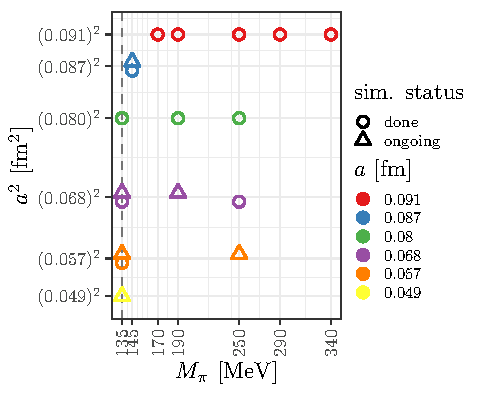
\includegraphics[height=7cm]{plots/ensembles_asquared_mpi}\hfill
  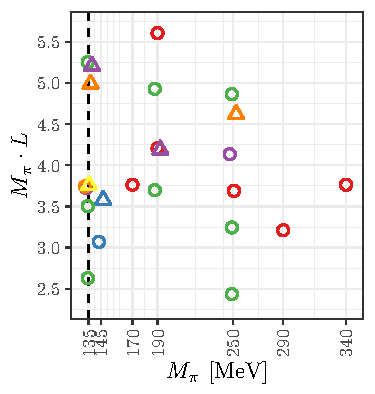
\includegraphics[height=7cm]{plots/ensembles_L_vs_mpi}
  \caption{Overview of all $N_f=2+1+1$ ETMC Wilson clover twisted mass ensembles as a function of the pion mass, the lattice spacing and $M_\pi \cdot L$. Points are slightly displaced either horizontally or vertically for visibility reasons. Lattice spacing and pion mass values are indicative.}
  \label{fig:ensemble_overview}
\end{figure}

\begin{SCfigure}
  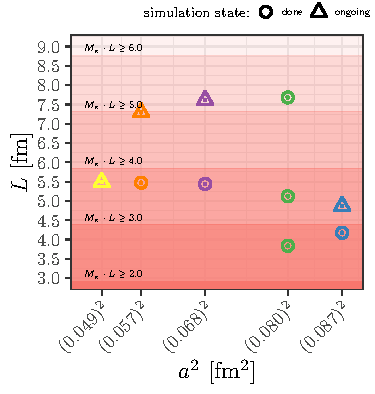
\includegraphics[width=0.5\linewidth]{plots/ensembles_phys_point}
  \caption{Overview of ETMC ensembles with $M_\pi \lesssim 147$ MeV as a function of the lattice spacing squared and the lattice volume in fermi. The different shaded regions indicate $M_\pi \cdot L$.}
  \label{fig:ensembles_phys_point}
\end{SCfigure}

% \begin{SCfigure}
%   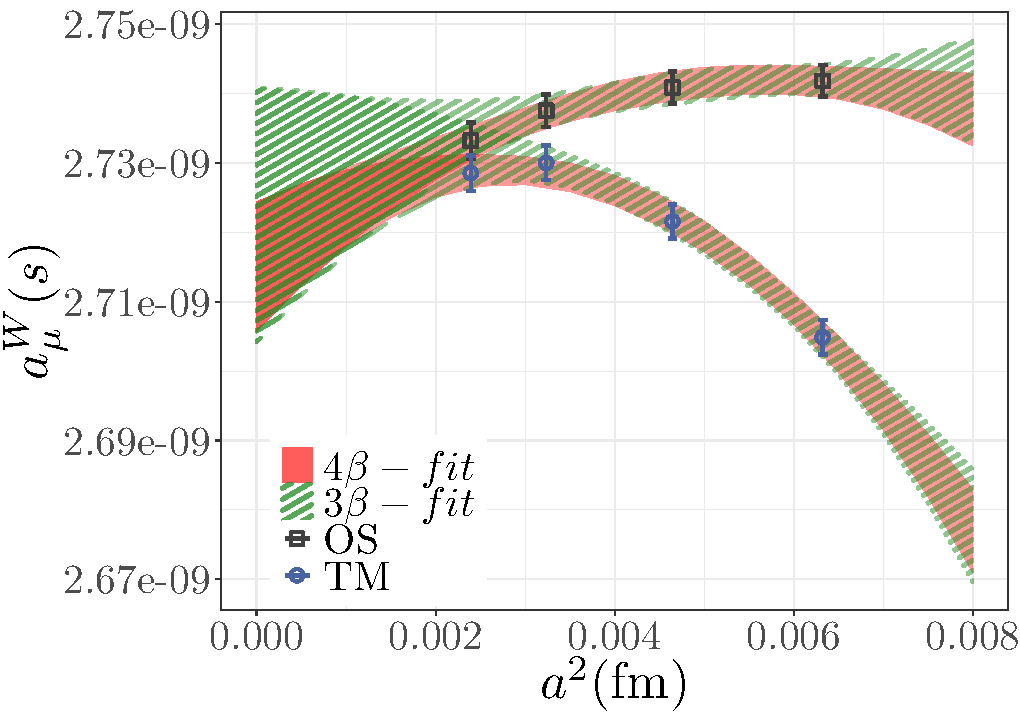
\includegraphics[width=\linewidth]{plots/amu_s_W_a4}
% \end{SCfigure}

\begin{figure}
  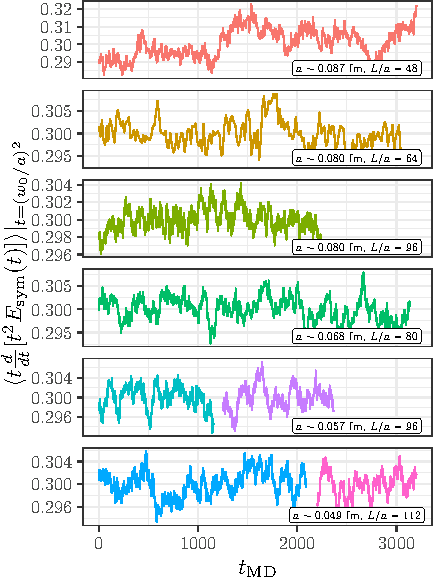
\includegraphics[width=0.49\linewidth,page=1]{../data/gf_observables/gf_observables_md_histories}
  \hfill
  \includegraphics[width=0.49\linewidth,page=2]{../data/gf_observables/gf_observables_md_histories}
  \caption{\textbf{Left:} Molecular dynamics histories for different ensembles close to or ar the physical point of the flow-time derivative of the gradient-flowed energy density, interpolated to the flow time where the ensemble average $t \frac{t}{dt} \lbrace t^2 \langle E(t) \rangle \rbrace = W(t)|_{t = w_0^2} = 0.3$. Only the first 2200 unit-length molecular dynamics units are shown in the histories whereas the histograms in the right sub-panels represent the full data sets. \textbf{Right:} Similar histories for the gradient-flowed topological charge in the clover definition evaluated at a flow time $t = w_0^2$. Lattice spacing values are indicative.}
  \label{fig:w0_Q}
\end{figure}

\section{Computational Setup}

Efficient usage of GPUs is achieved in tmLQCD via the QUDA library~\cite{Clark:2009wm,Babich:2011np}. As a first step in interfacing tmLQCD to QUDA \cite{Kostrzewa:2022hsv}  we offloaded the most expensive part of the HMC, i.e. the inversion of the various Dirac operators and the gauge force computation. In the last year, we further offloaded all computations of the fermionic force. In this way, tmLQCD can reach GPU utilizations over 70\% and even up to 90\% depending on the number of available CPU cores per GPU.
The evolution of the performance of this tmLQCD + QUDA setup is shown in the left panel of Figure~\ref{fig:quda_speedup}

\begin{figure}
  \includegraphics[width=0.5\linewidth,page=2]{plots/quda_speedup}
  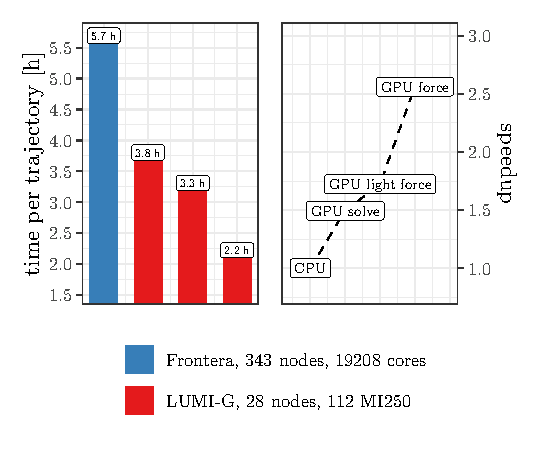
\includegraphics[width=0.5\linewidth,page=1]{plots/quda_speedup}
  \caption{\textbf{Left:} Time per unit length trajectory of tmLQCD + QUDA (green) for a $64^3 \cdot 128$ ensemble at the physical point compared to the machine it was originally generated on (purple) using tmLQCD + DD-$\alpha$AMG~\cite{Alexandrou:2016izb}. The different speedups correspond to increasing levels of QUDA offloading. \textbf{Right:} The same kind of comparison between tmLQCD + QUDA and tmLQCD + DD-$\alpha$AMG + QPhiX~\cite{QPhiX,Schrock:2015gik,QPhiX-github} running a $112^3 \cdot 224$ ensemble at the physical point on LUMI-G and Frontera, respectively.}
  \label{fig:quda_speedup}
\end{figure}

\section{Acknowledgements}
 {
  \small
  We would like to thank the QUDA developers for their tremendous work as well as the many pleasant and productive interactions during this and previous efforts.
  We thank the ETMC for the most enjoyable collaboration.
  For part of this work. S.B. and J.F. were supported by the H2020 project PRACE 6-IP (grant agreement No. 82376) and the EuroCC project (grant agreement No. 951740).
  This project was funded by the Deutsche Forschungsgemeinschaft (DFG, German Research Foundation) as part of the CRC 1639 NuMeriQS – project no. 511713970.
  This work was supported by the Deutsche Forschungsgemeinschaft (DFG, German Research Foundation) and the NSFC through the funds provided to the Sino-German Collaborative Research Center CRC 110 “Symmetries and the Emergence of Structure in QCD” (DFG Project-ID 196253076 - TRR 110, NSFC Grant No. 12070131001).
  We acknowledge support by the European Joint Doctorate program STIMULATE grant agreement No. 765048.
  We acknowledge support from projects NextQCD (EXCELLENCE/0918/0129) and "3D-Nucleon" (EXCELLENCE/0421/0043), co-funded by the European Regional Development Fund and the Republic of Cyprus through the Research and Innovation Foundation.
  We further acknowledge: The Gauss Centre for Supercomputing e.V. for funding this project through computing time on the GCS supercomputers SuperMUC and SuperMUC-NG at Leibniz Supercomputing Center as well as JUWELS Booster~\cite{JUWELS,BOOSTER} at the Jülich Supercomputing Centre.
  PRACE for awarding access to HAWK at HLRS within the project with Id Acid 4886.
  The Swiss National Supercomputing Centre (CSCS) and the EuroHPC Joint Undertaking for awarding access to the LUMI supercomputer, owned by the EuroHPC JU, hosted by CSC and the LUMI consortium through the Chronos programme under project IDs CH17-CSCS-CYP and CH21-CSCS-UNIBE as well as EuroHPC under project ID EHPC-REG-2021R0095.
  The Texas Advanced Computing Center (TACC) at The University of Texas at Austin for providing HPC resources on Frontera~\cite{FRONTERA} (Project ID PHY21001).
  The EuroHPC Joint Undertaking for awarding access to the Luxembourg national supercomputer MeluXina.
  The University of Bonn for access to the Bender and Marvin clusters as well as support by the HRZ-HPC team.
  The open-source packages tmLQCD~\cite{Jansen:2009xp,Abdel-Rehim:2013wba,Deuzeman:2013xaa,Kostrzewa:2022hsv,tmLQCD_mg_tune}, LEMON~\cite{Deuzeman:2011wz}, DD-$\alpha$AMG~\cite{Frommer:2013fsa,Alexandrou:2016izb,Bacchio:2017pcp,Alexandrou:2018wiv}, QPhiX~\cite{qphix13,qphix14,qphix16,Schrock:2015gik} and QUDA~\cite{Clark:2009wm,Babich:2011np,Clark:2016rdz} have been used.
 }

\bibliographystyle{JHEP}
{\footnotesize
  \bibliography{bibliography}
}

\end{document}
